\subsection{Data Pipeline}\label{sec:data-pipeline}
Two datasets are used in this thesis. The first is the TTF futures dataset, which is used to train and evaluate the model. The second is the TTF options dataset, which provides the market prices for the benchmark in Sec.~\ref{sec:pricing-setup}.

\subsubsection{Futures Data}\label{sec:futures-data}
The futures data was obtained from BASF's Bloomberg infrastructure and covers
TTF natural gas futures for the first three nearby contracts between January
2010 and April 2026. The data is distributed as three files: contract prices, contract metadata, and monthly listings of active contracts.

\textbf{Daily settlement prices.} This file provides the price history of the contracts in the dataset.  Each contract is observed once per trading day, identified by contract symbol and trading date. Each record contains opening, high, low and daily closing prices in EUR/MWh, trading volume and open interest. Coverage of these fields varies considerably with how actively a contract was traded and how far from expiry it is. The closing price is the exception and is available throughout the whole dataset. Additionally, it falls outside the intraday high–low range for \num{7712} of \num{25884}  records, or 29.8\%. The deviation is small in most cases, with a median of \num{0.10} EUR/MWh, but reaches up to \num{42.26} EUR/MWh. The latter confirms that it is a settlement price set by the exchange rather than a price at which trading occurred.

\textbf{Contract metadata.} This file provides static attributes per unique contract in the dataset. The expiry date provided per record is used to rank contracts by time to maturity in Sec.~\ref{sec:m1-construction}. All contracts in the dataset are physically delivered instruments traded on ICE Endex and quoted in EUR/MWh. First and last trading dates, notice dates and delivery dates are also recorded.

\textbf{Contract listings.} This file records which contracts were active on the market, as monthly snapshots taken on the first calendar day of each month. Each contract is observed once per snapshot. Together with the expiry dates, the listings determine which contract is the front month on a given date, as described in Sec.~\ref{sec:m1-construction}.

\subsubsection{Front-Month Series Construction}\label{sec:m1-construction}
As described in Sec.~\ref{sec:futures-data}, the contract listings and the
contract metadata each hold part of the information required to identify
the front-month contract. The listings record which contracts were active in a
given month, while the metadata records when each contract expires. Therefore, the expiry dates were joined onto the listings by contract symbol. As a result, each listing record carries the expiry date of the contract it refers to. 

The contracts were then sorted by expiry date within each monthly snapshot and the earliest-expiring one was kept. \footnote{Trading in a TTF futures
contract ceases two UK business days before the first day of the delivery month.} This gives the front-month contract for that month. Since the snapshots are monthly but the series must be daily, each trading day was assigned the front-month contract from the most recent snapshot on or before that day.
The settlement price of the selected contract was then added for each trading day, matching on trading date and contract symbol. The trading days without an available settlement price were discarded. The resulting series contains \num{3998} trading days spanning 2010-01-04 to 2026-04-24, with settlement prices ranging from \num{3.509} to \num{339.196}~EUR/MWh.

Since the front-month contract is replaced at each expiry, the series is not the price history of a single instrument. Returns spanning a contract transition reflect the change in the price level as well as the difference between the two contracts. Across the \num{195} transition days in the sample, the standard deviation of daily log returns is \num{0.071}, compared to \num{0.037} on all other days. When the transition days are excluded, excess kurtosis falls from \num{14.91} to \num{14.65}, and skewness from \num{0.70} to \num{0.26}. \footnote{Skewness and excess kurtosis are computed with the sample estimators $g_1$ and $g_2$ of Eq.~\eqref{eq:g1-g2}.} Transition days contribute little to the tail weight of the series, but they are responsible for most of its positive skew. 


The transition effect described above is preserved and quantified rather than removed, since restricting the analysis to a single contract would reduce the sample to a few months.

\subsubsection{Return Definition}\label{sec:return-definition}
The original Fin-GAN input series is built from two returns per day \parencite{vuleticFinGANForecastingClassifying2024}. The first is the intraday return, from the opening to the closing price and the second is the overnight return, from one closing price to the next opening
price. The return of the corresponding sector ETF is then subtracted from each entry. This isolates the part of the movement specific to the asset.

Neither step has been adopted for the TTF futures dataset. The two-return scheme requires opening and closing prices that are both traded prices. As shown in Sec.~\ref{sec:futures-data}, the daily price in this dataset is a settlement price set by the exchange. A return computed between the opening trade and the settlement price would therefore combine two different price concepts.

Additionally, the excess-return step requires a benchmark that leaves a meaningful residual when subtracted. In the case of equities, subtracting the sector ETF return removes the market-wide component and leaves the movement specific to the individual stock. European natural gas has no comparable instrument.

As a substitute, the second nearby contract was considered. However, the difference between the first and second nearby returns is a calendar spread return, as described in Sec.~\ref{sec:futures}. A model that is trained on it would learn how the gap between two contracts moves, not how the gas price itself moves. Option payoffs depend on the price level at expiry, so a model trained on spread returns could not be used to price options.

Therefore, the dataset was constructed from daily logarithmic returns of the front-month settlement price. Returns are approximately stationary and therefore comparable across the sample period. Additionally, log returns are additive across time and allow price levels to be recovered exactly from simulated returns. The latter is required for the Monte Carlo procedure
in Sec.~\ref{sec:pricing-setup}.

\begin{equation}\label{eq:logreturn}
    x_t = \log\!\left(\frac{P_t}{P_{t-1}}\right),
\end{equation}
where $P_t$ is the front-month settlement price on trading day $t$.
The transformation gives \num{3997} return observations.

\subsubsection{Data Split}\label{sec:data-split}
The return series was split chronologically into training (80\%), validation (10\%), and test (10\%) sets using the proportions of \textcite{vuleticFinGANForecastingClassifying2024}. Training covers 2010-01-05 to 2023-01-18
validation 2023-01-19 to 2024-09-04 (\num{399} returns), and test
2024-09-05 to 2026-04-24 (\num{401} returns). The chronological split was explicitly used to avoid look-ahead bias. Following the current split, the 2021 to 2022 price disruption discussed in Sec.~\ref{sec:gas-markets} falls entirely within the training period, and the 2026 disruption falls entirely within the test period, as seen in Fig.~\ref{fig:ttf-price-split}.

Sliding window matrices were constructed for each split separately, so that no window spans a split boundary. The window was moved forward by one trading day.

\begin{figure}[htbp]
    \centering
    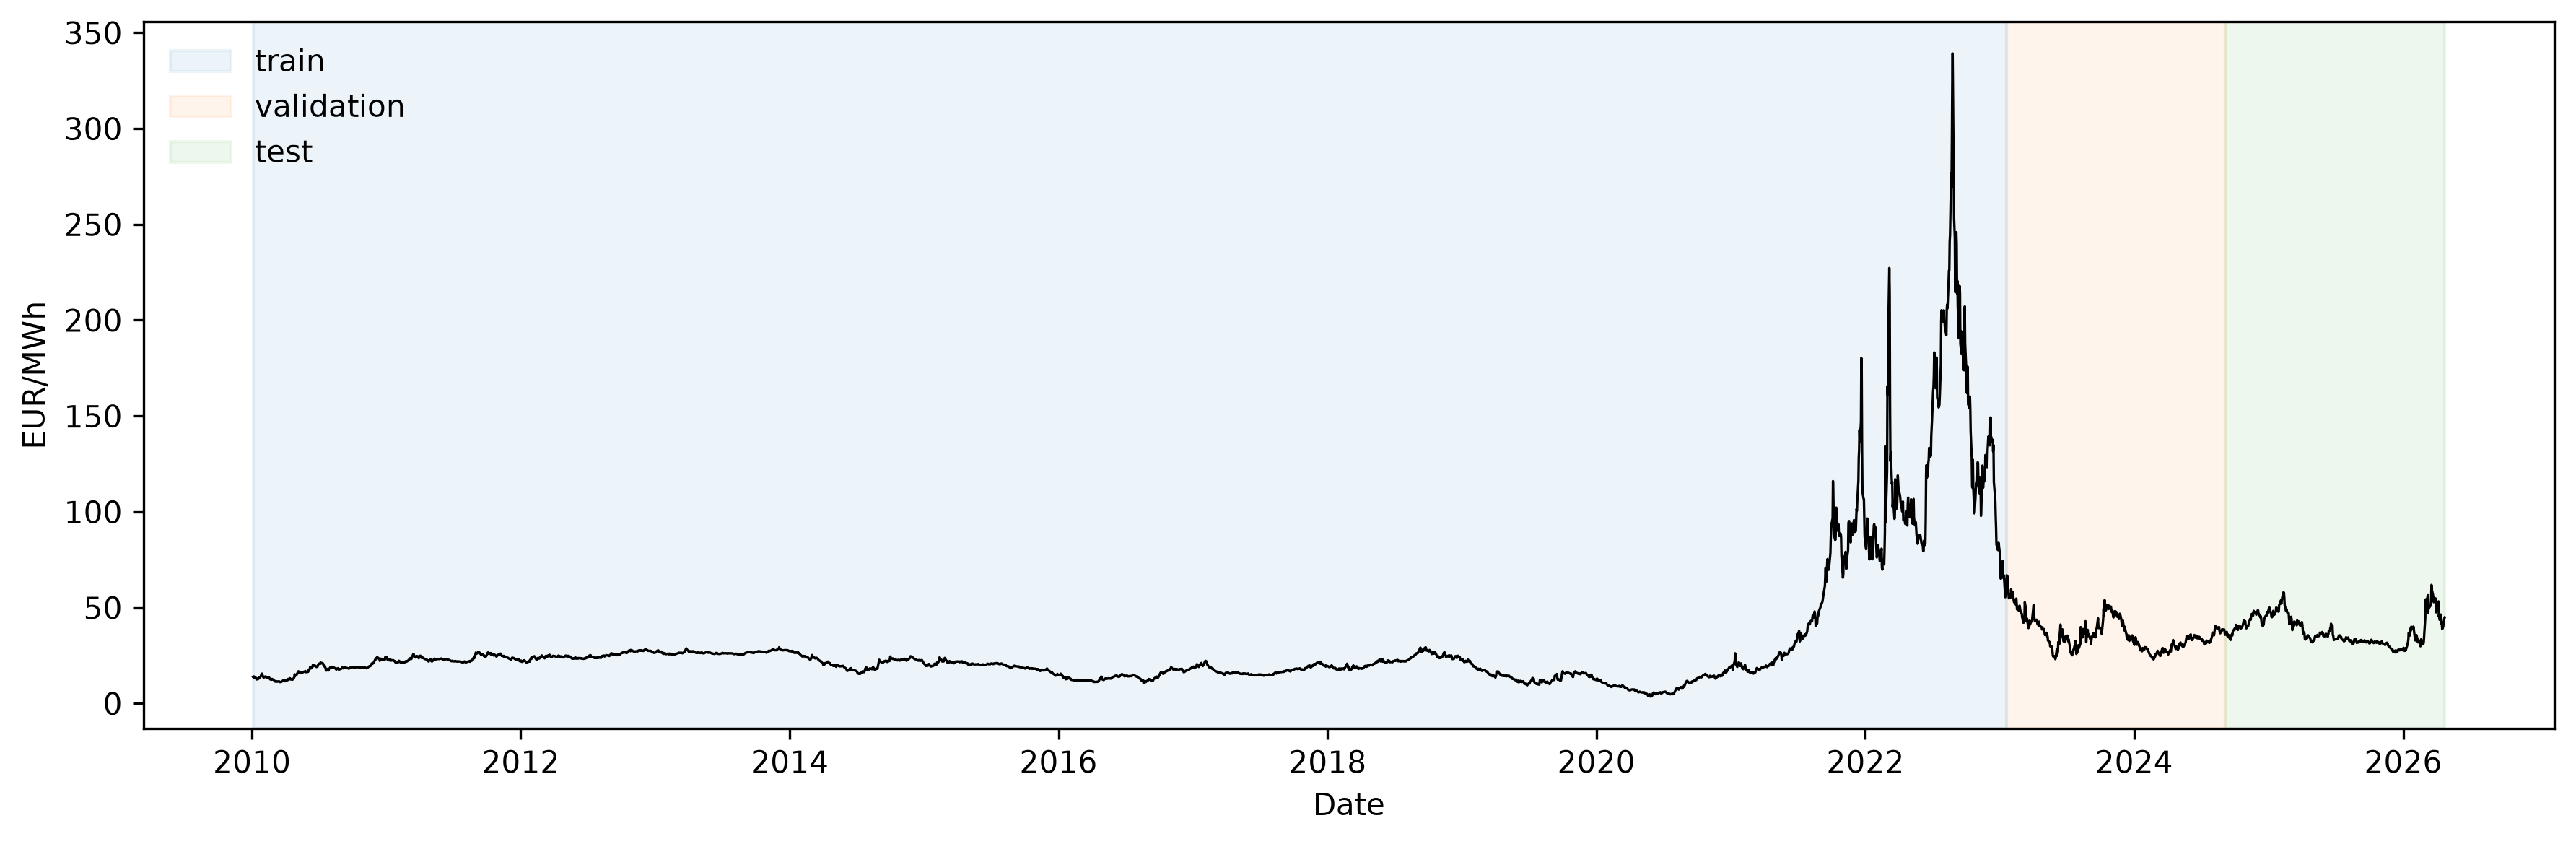
\includegraphics[width=\textwidth]{figures/ttf_price_split.png}
    \caption{TTF train, validation and test data split}
    \label{fig:ttf-price-split}
\end{figure}

\subsubsection{Options Data}\label{sec:options-data}
